%!TEX root = ../thesis.tex

% \pagebreak[4]
% \hspace*{1cm}
% \pagebreak[4]
% \hspace*{1cm}
% \pagebreak[4]

\chapter{Extensions}

\graphicspath{ {Chapter4/Chapter4Figs/PNG/}
  {Chapter4/Chapter4Figs/PDF/} {Chapter4/Chapter4Figs/} }

Dans le dernier chapitre, nous avons vu une nouvelle méthode permettant
combiner des outils de déformation à base de cage. Cette méthode utilise un
nouveau type d'outil, la cage de contrôle d'influence. Cet outil est composé
de deux cages. L'une dite cage d'influence, elle délimite la zone de l'espace
sous l'influence de la déformation. L'autre dite de contrôle, elle permet à
l'utilisateur de contrôler la déformation à appliquer.

Nous avions choisi de travailler avec une cage comme outil de contrôle puisque
nous voulions une méthode de mélange d'outils de déformation à base de cage.
Mais rien ne nous empêche de changer la nature de cette cage de contrôle. Pour
généraliser un peu plus ces propos, nommons la cage de contrôle \textit{outil
de contrôle}. A partir du moment où un outil (point, courbe, face) nous permet
de définir une cage d'influence, nous pouvons l'utiliser comme outil de
contrôle.

Clarifions un peu ces explications. Imaginons que notre outil de contrôle soit
un point. Pour obtenir la cage d'influence associée à ce point, nous pouvons
construire un polygone régulier (de résolution quelconque) de façon à ce que
l'isobarycentre de ce polygone soit l'outil de contrôle (Figure \ref{EXTPoi}).
Le lien entre l'outil de contrôle et la cage d'influence s'établit sur le
principe que l'outil de contrôle doit rester l'isobarycentre de la cage
d'influence. La modification de la position de l'outil de contrôle implique une
modification de la position des sommets de la cage d'influence (par
invariance de l'association).

\begin{figure}[ht]
\begin{center}
  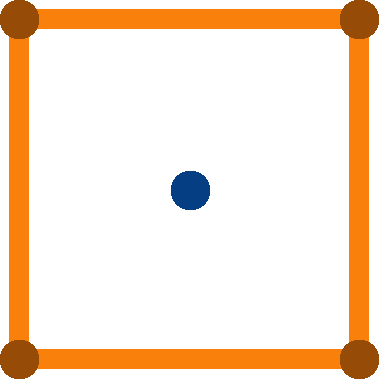
\includegraphics[scale=0.3]{OutilControle-Point-4}
  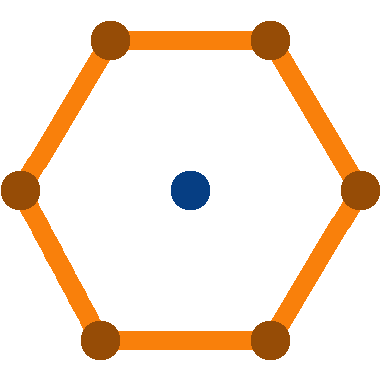
\includegraphics[scale=0.3]{OutilControle-Point-6}
  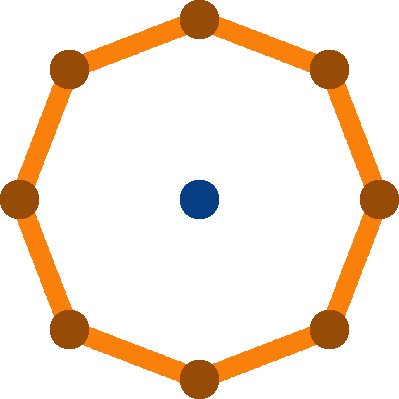
\includegraphics[scale=0.3]{OutilControle-Point-8}

  \caption[Cages d'influence à partir d'un point] {Différentes cages
d'influence créées à partir d'un point comme outil de contrôle}
  \label{EXTPoi}

\end{center}
\end{figure}
